\section{Bridging the Gap of doing and learning} \label{chap_reflection}

In this Chapter, I will discuss my experiences and learnings from working with \gls{ns}
and \gls{ca} during my research. I will use the "5-ways" framework to structure my
reflections, providing insights into my thinking, managing, modeling, working, and
supporting aspects of the developing approaches that were the topic of my research.
Through this chapter, I hope to demonstrate the value of NS and its contribution to my
knowledge in software engineering.

\begin{figure}[H]
    \centering
    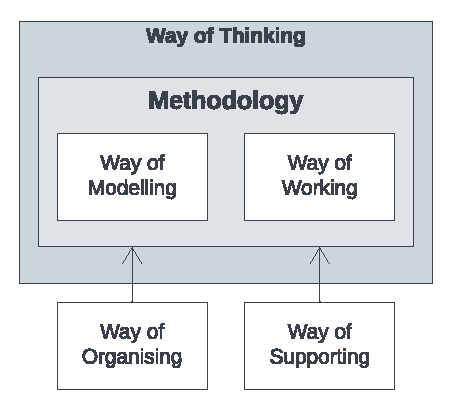
\includegraphics[width=0.5\textwidth]{figures/5ways.pdf}
    \caption[The Five Way Framework]{The Five Way Framework, inspired by \textcite{dietz_enterprise_2020}}
    \label{fig_5ways}
\end{figure}

\subsection{Way of Thinking}

One of the aspects of \gls{ns} is the characteristics of code generation. In my Job as a
Domain Architect, I was involved in the development of software products based on the
\gls{mdd} paradigm. My early experiences made me very sceptical about this approach. The
theory of \gls{ns} taught me to better understand the reasoning and characteristics of
code generation, on which I then realized that my skepticism was more about the process
caused as an effect on the implementation of the \gls{mdd}. The knowledge of \gls{ns}
helped me to gain a more clear vision. This currently helps me push the roadmap on the
\gls{mdd} framework in the right direction.

\subsection{Way of Managing}


\subsection{Way of Modeling}

I considered multiple modeling languages in order to explain the implementation concepts
of the artifact. One of which was the idea of using Archimate, but decided otherwise as I
wanted to use a language that could be interpreted by a broader audience. I even
considered just using \emph{boxes and arrows}, but eventually decided on the UML2 standard
as it is an official modeling language.

\subsection{Way of Working}

The topic of \gls{ns} re-ignited my passion for software engineering and the aspects of
designing and creating, -what I would previously mention as maintainable and qualitative.
\gls{ns} Taught me that it was in fact about software evolvability and stability. And on
top of that, \gls{ns} contributed greatly to my knowledge in doing so.

I very much enjoyed designing and creating the C\# artifacts. In hindsight, I enjoyed it
so much that I probably put in much more effort than was needed. This was also because I
was very curious about the aspects of code generation, the effect of code generation on
stable and evolvable artifacts and the characteristics of meta-circularity. I'm confident
to say that I could have reached the same conclusions that are described in this Thesis,
with a single, manually built Restful C\# artifact.

The \gls{ns} theorems are so nicely and abstractly formulated, that it ascends the domain
of software engineering. During the masterclasses, we learned about applications of
\gls{ns} in the areas of Firewalls, Document management systems and Evolvable Business
Processes. I experienced also benefits in structuring and maintaining my Thesis document
using \gls{vscode} and Latex. 

\subsection{Way of Suporting}

At the beginning of my research, I received a thorough introduction to the \gls{ns}
Theories and the Prime Radiant tooling from an employer at NSX. This introduction was
extremely helpful in gaining a better understanding of the fundamentals of \gls{ns}. It
also inspired me to consider the code-generation aspects of the methodology, as well as
the use of expanders, which are valuable for consistently delivering software artifacts
with great precision. One thing and another has led to the decision to create the
artifacts as described in this thesis.

For the writing of the Thesis, I decided to use Latex. I quickly discovered that Overleaf
was one of the most popular editors. Nevertheless, I continued my search since I did not
like the idea of being dependent on online tooling for writing my thesis. Although offline
working is possible, doing so is very rudimentary without having the complete experience. At
some point, I decided to experiment with my favorite code editor \gls{vscode}, and
with the help of a latex package manager and some VSCode plugins I was able to create
a fully-fledged Latex Editor in \gls{vscode}, with all it's benefits. There was even a
plugin available that allowed me to use the spellchecker Grammarly while writing and
modifying the .tex files.

Using Latex was a real eye-opener, and very relatable to my research as it allowed me to
adhere to most of the \gls{ns} principles while writing and maintaining my Thesis.
